\documentclass{article}
\usepackage[utf8]{inputenc}
\usepackage[english]{babel}
\usepackage[T1]{fontenc}

\usepackage{amsfonts}
\usepackage{amsmath}
\usepackage{amssymb}
\usepackage{tikz}
\usepackage{graphicx}
\usepackage{color}
\usepackage{enumitem}
\usetikzlibrary{arrows}
\usepackage{framed}
\usepackage{arydshln}
\usepackage{multirow}
\usepackage{mathtools}


% no indent
\setlength\parindent{0pt}

% commands
\usepackage{amsthm}
\theoremstyle{definition}
\newtheorem{definition}{Definition}[section]
\newtheorem{remark}{Remark}

\newcommand{\real}{\mathbb{R}}
\newcommand{\tspace}{\mathbb{T}}
\newcommand{\vecspace}{\mathbb{V}}
\newcommand{\ovec}{}

\newcommand{\todo}[1]{\textcolor{red}{TODO: #1\\}}

\title{Structures en apprentissage profond.\\ On structures in deep learning}

\begin{document}

\section{Definitions and disambiguations}

\todo{Explain why we do rigourous defintions and argue on the added value}
In this section we recall and define the notions we will be using in this manuscript.

\subsection{Tensors}

Vector spaces considered in this thesis are assumed to be finite-dimensional and over the field of real numbers $\real$.

\begin{definition}\textbf{Tensor space}\\
We define a \emph{tensor space} $\tspace$ of rank $r$ as a cartesian product of $r$ vector spaces, equipped with the coordinate-wise sum and the mono-linear outer product.

Its \emph{shape} is denoted $n_1 \times n_2 \times \cdots \times n_r$, where the $\{n_k\}$ are the dimensions of the vector spaces.
\end{definition}

For notational conveniency, we will often abusively confound vector spaces with tensor spaces of rank $1$, and matrix spaces with tensor spaces of rank $2$.

\begin{definition}\textbf{Tensor}\\
A \emph{tensor} $t$ is an object of a tensor space.

The \emph{shape} of $t$, which is the same as the shape of the tensor space it belongs to, is denoted $n_1^{(t)} \times n_2^{(t)} \times \cdots \times n_r^{(t)}$.
An \emph{entry} is denoted $t[i_1, i_2, \ldots, i_r]$.
\end{definition}

When using an index $i_k$ for an entry of a tensor $t$, we implicitly assume that $i_k \in \{1, 2, \cdots, n_k^{(t)}\}$ if nothing is precised.

\begin{definition}\textbf{Slice}\\
A \emph{slice} of a tensor $t$, along the last ranks $\{r_1, r_2, \ldots, r_s\}$, and indexed by  $\{i_{r_1}, i_{r_2}, \cdots, i_{r_s}\}$, is the tensor $t'$ of rank $r-s$ such that
\begin{align*}
t'[i'_1, i'_2, \ldots, i'_{r-s}] &= t[i'_1, i'_2, \ldots, i'_{r-s}, i_{r_1}, i_{r_2}, \ldots, i_{r_s}] \\
\text{ i.e. } \quad t' :&= t[:,:, \ldots, :, i'_{r-s}, i_{r_1}, i_{r_2}, \ldots, i_{r_s}]
\end{align*}
We denote $t_{i_{r_1} i_{r_2} \cdots i_{r_s}}$. Hence its shape is $n_1^{(t)} \times n_2^{(t)} \times \cdots \times n_{r-s}^{(t)}$.
\end{definition}

\begin{definition}\textbf{Flattening}\\
A \emph{flatten} operation is a bijection $f$ between a tensor space $\tspace$ of rank $r$ and an $n$-dimensional vector space $\vecspace$ such that
\begin{gather*}
\left\{
  \begin{array}{l}
  \displaystyle \prod_{k=1}^r n_k = n \\
  \forall t \in \tspace, f(t)[\displaystyle \sum_{p=1}^r \left( \prod_{k=p+1}^r n_k \right) i_p ] = f(t[i_1, i_2, \ldots, i_r])
  \end{array}
\right.
\end{gather*}
An inverse operation is called a \emph{de-flatten} operation.
\end{definition}

\begin{definition}\textbf{Reshaping}\\
A \emph{reshape} operation is a bijection $g$ defined on a tensor space $\tspace = \displaystyle \prod_{k=1}^r \vecspace_k$ such that its basis vector spaces $\{\vecspace_k\}$ are either de-flattened or flattened by contiguous groups $\{\displaystyle \prod_{p=0}^{s-1} \vecspace_{s_0+p}\}$.
\end{definition}

\begin{definition}\textbf{Contraction}\\
A \emph{tensor contraction} between two tensors, along ranks of same dimensions, is defined as the tensor equivalent of the dot product operation.

More precisely, let $\tspace_1$ a tensor space of shape $n_1^{(1)} \times n_2^{(1)} \times \cdots \times n_{r_1}^{(1)}$, and $\tspace_2$ a tensor space of shape $n_1^{(2)} \times n_2^{(2)} \times \cdots \times n_{r_2}^{(2)}$, such that $\forall k \in \{1, 2, \ldots, s\}, n_{r_1-(s-k)}^{(1)} = n_k^{(2)}$, then the tensor contraction between $t_1 \in \tspace_1$ and $t_2 \in \tspace_2$ is defined as:
\begin{gather*}
\left\{
  \begin{array}{l}
    t_1 \otimes t_2 = t_3 \in \tspace_3 \text{ of shape } n_1^{(1)} \times \cdots \times n_{r_1-s}^{(1)} \times n_{s+1}^{(2)} \times \cdots \times n_{r_2}^{(2)}
    \text{ where} \\
    t_3[i_1^{(1)}, \ldots, i_{r_1-s}^{(1)}, i_{s+1}^{(2)}, \ldots, i_{r_2}^{(2)}] = \\
    \displaystyle \sum_{k_1, \ldots, k_s}
    t_1[i_1^{(1)}, \ldots, i_{r_1-s}^{(1)}, k_1, \ldots, k_s] \hspace{2pt}
    t_2[k_1, \ldots, k_s, i_{s+1}^{(2)}, \ldots, i_{r_2}^{(2)}]
  \end{array}
\right.
\end{gather*}
\end{definition}

\begin{remark}\textbf{Covariant and contravariant indices}\\
Indices of the left handed operand $t_1$ that are not contracted are called \emph{covariant} indices. Those that are contracted are called \emph{contravariant} indices. For the right operand $t_2$, the naming convention is the opposite. Using subscript notation for covariant indices and superscript notation for contravariant indices, the previous tensor contraction can be written using the Einstein summation convention as:
\begin{gather*}
t_1 \hspace{0pt}_{i_1^{(1)} \cdots i_{r_1}^{(1)} } \hspace{0pt}^{ k_1 \cdots k_s} \otimes
t_2 \hspace{0pt}_{ k_1^{\phantom{(}} \cdots k_s^{\phantom{(}}} \hspace{0pt}^{i_{s+1}^{(2)} \cdots i_{r_2}^{(2)}} =
t_3 \hspace{0pt}_ {i_1^{(1)} \cdots i_{r_1}^{(1)} } \hspace{0pt}^{i_{s+1}^{(2)} \cdots i_{r_2}^{(2)}}
\end{gather*}
\end{remark}

Dot product $u_k v^k = \lambda $ and matrix product $A_i\hspace{0pt}^k B_k\hspace{0pt}^j = C_i\hspace{0pt}^j$ are common examples of tensor contractions.

\begin{remark}\textbf{Matrix product equivalence}\\
Using a reshaping that groups all covariant indices into a single index and all contravariant indices into another single index, any tensor contraction can be rewritten as a matrix product.
\end{remark}

\begin{definition}\textbf{Convolution}\\
The \emph{$n$-dimensional convolution} between $t_1 \in \tspace_1$ and $t_2 \in \tspace_2$, where $\tspace_1$ and $\tspace_2$ are of the same rank $n$, is defined as:
\begin{gather*}
\left\{
  \begin{array}{l}
t_1 \ast_r t_2 = t_3 \in \tspace_1 \\
t_3[i_1, \ldots, i_n] = \displaystyle \sum_{k_1, \ldots, k_n} \widetilde{t_1}[i_1 - k_1, \ldots, i_n - k_n] \hspace{2pt} t_2[k_1, \ldots, k_n] \\
\text{where } \widetilde{t_1}[p_1, \ldots, p_n] =
  \begin{cases}
  t_1[p_1, \ldots, p_n] & \text{if } \forall q, 1 \le p_q \le n_q(t_1) \\
  0 & \text{otherwise}
  \end{cases}
  \end{array}
\right.
\end{gather*}
\end{definition}

\subsection{Neural Networks}

We denote by $I_f$ the \textit{domain of definition} of a function $f$ ("I" for "input") and by $O_f = f(I_f)$ its \textit{image} ("O" for "output"), and we represent it as $I_f~\xrightarrow{f}~O_f$.

An activation function $h$ defined from a tensor space to itself is a $1$-d function applied dimension-wise and we use the functional notation $h(v)[i_1, i_2, \ldots, i_r] = h(v[i_1, i_2, \ldots, i_r])$.

\begin{definition}\textbf{Neural network}\\
\label{nndef}
{Let $F$ be a function such that $I_f$ and $O_f$ are vector or tensor spaces.\\
$F$ is a \emph{functional formulation} of a \emph{neural network} if there are a series of linear or affine functions $(g_k)_{k=1,2,..,L}$ and a series of non-linear derivable activation functions $(h_k)_{k=1,2,..,L}$ such that:
\begin{gather}
\left\{
  \begin{array}{l}
    \forall k \in \{1,2,..,L\}, f_k = h_k \circ g_k, \\
    I_F = I_{f_1} \xrightarrow{f_1} O_{f_1} \cong I_{f_2} \xrightarrow{f_2} \dots \xrightarrow{f_L} O_{f_L} = O_F, \\
    F = f_{L} \circ ... \circ f_{2} \circ f_1
  \end{array}
\right.
\end{gather}
The couple $(g_k, h_k)$ is called the \emph{$k$-th layer} of the neural network.
For $\ovec{x} \in I_f$, we denote by $\ovec{x_k} = f_k \circ ... \circ f_{2} \circ f_1 (\ovec{x})$ the \emph{activations} of the $k$-th layer.
}
\end{definition}

\begin{remark}\textbf{Bias}\\
Affine functions $\widetilde{g}$ can be written as a sum between a linear function $g$ and a constant vector $b$. For notational conveniency, we only consider linear functions in this section. $b$ is called the \emph{bias}. Its role is to augment the expressivity of the neural network's family of functions.
\end{remark}

\begin{definition}\textbf{Connectivity matrix}\\
Any linear function $g$ is characterized by a \emph{set of parameters} $\Theta_g$, that we order arbitrarily in the dimensions of a vector $\theta_g$. Without loss of generality subject to a flattening, let's suppose $I_g$ and $O_g$ are vector spaces. Then there exists a \emph{connectivity matrix}~$W_g$, for which:
\begin{gather}
\left\{
\begin{array}{l}
  \forall \ovec{x} \in I_g, g(\ovec{x}) = W_g\ovec{x}\\
  \forall (i,j),
    \begin{cases}
      \exists w \in \Theta_g, W_g[i,j] := w \\
      \text{ or } W_g[i,j] = 0
    \end{cases}
\end{array}
\right.
\end{gather}
\end{definition}

\begin{remark}\textbf{Biological inspiration}\\
A \emph{(computational) neuron} is a computational unit that is biologically inspired. Each neuron should be capable of:
\begin{enumerate}
\item receiving modulated signals from other neurons and aggregate them,
\item applying to the result a derivable activation,
\item passing the signal to other neurons.
\end{enumerate}
That is to say, each domain $\{I_{f_k}\}$ and $O_F$ can be interpreted as a layer of neurons, with one neuron for each dimension. The connectivity matrices $\{W_k\}$ describe the connexions between each successive layers. A neuron is illustrated on Figure~\ref{fig:neuron}.
\end{remark}

\begin{figure}[h]
\centering
\begin{tikzpicture}
\draw (0,0) -- (4,0) -- (4,4) -- (0,4) -- (0,0);
\node at (2,2){placeholder};
\end{tikzpicture}
\caption{A neuron}
\label{fig:neuron}
\end{figure}

\begin{definition}\textbf{Weights}\\
The \emph{weights} of the $k$-th layer of a neural network, denoted $\Theta_k$, are defined as the set of parameters of its linear part.
A weight that appears multiple times in $W_k$ is said to be \emph{shared}. Two parameters of $W_k$ that share a weight are said to be \emph{tied}.
\end{definition}

\begin{remark}\textbf{Training}\\
Usually, a \emph{loss} function $\mathcal{L}$ penalizes the output $x_L = F(\ovec{x})$. Its gradient w.r.t.~$\theta_k$, denoted $\vec{\bigtriangledown}_{\theta_k}$, is used to update the weights via an optimization algorithm based on gradient descent and a learning rate $\alpha$, that is:
\begin{gather}
\theta_k^{\text{new}} = \theta_k^{\text{old}} - \alpha \cdot \vec{\bigtriangledown}_{\theta_k}
\end{gather}
where $\alpha$~can be a scalar or a vector, and $\cdot$~can denote outer or pointwise product. $\alpha$ and~$\cdot$~ depend on the optimization algorithm.
\end{remark}

\begin{remark}\textbf{Linear complexity}\\
{Thanks to the chain rule, $\vec{\bigtriangledown}_{\theta_k}$ can be computed using gradients that are w.r.t. $\ovec{x_k}$, denoted $\vec{\bigtriangledown}_{x_k}$, which in turn can be computed using gradients w.r.t. outputs of the next layer $k+1$, up to the gradients given on the output layer.

That is:
%$$
%\left\{
%\begin{array}{l}
\begin{align}
  \vec{\bigtriangledown}_{\theta_k} & = J(\ovec{x_k})_{\theta_k} \vec{\bigtriangledown}_{x_k} \\
  \begin{split}
  \vec{\bigtriangledown}_{x_k} & = J(\ovec{x_{k+1}})_{x_k} \vec{\bigtriangledown}_{x_{k+1}} \\
  \vec{\bigtriangledown}_{x_{k+1}} & = J(\ovec{x_{k+2}})_{x_{k+1}} \vec{\bigtriangledown}_{x_{k+2}} \\
  \quad \quad \ldots\\
  \vec{\bigtriangledown}_{x_{L-1}} & = J(\ovec{x_{L}})_{x_{L-1}} \vec{\bigtriangledown}_{x_{L}}
  \label{eq:bp}
  \end{split}
\end{align}
Obtaining,
\begin{align}
  \vec{\bigtriangledown}_{\theta_k} = J(\ovec{x_k})_{\theta_k} (\prod_{p=k}^{L-1} J(\ovec{x_{p+1}})_{x_p}) \vec{\bigtriangledown}_{x_L}
\end{align}
%\end{array}
%\right.
%$$
where $J(.)_{\text{wrt}}$ are the respective jacobians which can be determined with the layer's expressions and the $\{x_k\}$.

This allows to compute the gradients with a complexity that is linear with the number of weights, instead of being quadratic if it were done with the difference quotient expression of the derivatives.}
\end{remark}

\begin{remark}\textbf{Neural interpretation}\\

We can remark that \eqref{eq:bp} rewrites as
\begin{align}
  \begin{split}
  \vec{\bigtriangledown}_{x_k} & = J(\ovec{x_{k+1}})_{x_k} \vec{\bigtriangledown}_{x_{k+1}} \\ 
                               & = J(h(x'_k))_{x'_k} J(W_k x_k)_{x_k} \vec{\bigtriangledown}_{x_{k+1}}
                               %& = \text{diag}( h_k'(W_k x_k) ) W_k \vec{\bigtriangledown}_{x_{k+1}}
  \end{split}
\end{align}
where $x'_k = W_k x_k$, and these jacobians can be expressed as:
\begin{align}
  \begin{split}
  J(h(x'_k))_{x'_k} & [i,j] = \delta_i^j h'(x'_k[i])\\
  J(h(x'_k))_{x'_k} & = I \hspace{2pt} h'(x'_k)
  \end{split}\\
  J(W_k x_k)_{x_k} & = W_k^T
\end{align}
That means that we can write $\vec{\bigtriangledown}_{x_k} = (\widetilde{h}_k \circ \widetilde{g}_k)(\vec{\bigtriangledown}_{x_{k+1}})$ such that the connectivity matrix $\widetilde{W}_k$ is obtained by transposition. This can be interpreted as gradient calculation being a \emph{back-propagation} on the same neural network, in opposition of the \emph{forward-propagation} done to compute the output.
\end{remark}

\begin{definition}\textbf{Dense layer}\\
A \textit{dense layer} $(g,h)$ is a layer such that
$$
\left\{
\begin{array}{l}
  I_g \mbox{ and } O_g \mbox{ are vector spaces} \\
  \forall w \in \Theta_g, \exists! (i, j), W_g[i,j] := w \\
  | \Theta_g | = n_1^{(W_g)}n_2^{(W_g)}
\end{array}
\right.
$$
\end{definition}

That is, there is no weight sharing, and all possible connections in the connectivity matrix exist. When some connections don't exist, we have the following type of layer:

\begin{definition}\textbf{Partially connected layer}\\
A \textit{partially connected layer} is a layer such that
$$
\left\{
\begin{array}{l}
  I_g \mbox{ and } O_g \mbox{ are vector spaces}\\
  \exists (i,j), \forall w \in \Theta_g, W_g[i,j] :\neq w
\end{array}
\right.
$$
\end{definition}

\begin{definition}\textbf{Convolutional layer}\\
A \textit{$n$-dimensional convolutional layer} $(g,h)$ is a layer such that there is a \textit{weight kernel} tensor $w$ of rank $n+2$ for which
$$
\left\{
\begin{array}{l}
  I_g \mbox{ and } O_g \mbox{ are tensor spaces of rank }n+1 \\
  \forall x \in I_g, g(x) = (g(x)_q = \sum\limits_p{x_p \ast_n w_{pq}})_{\forall q}
\end{array}
\right.
$$
where $p$ and $q$ index the last ranks and $\ast_n$ denotes the n-d convolution. The tensor slices indexed by $p$ and $q$ are typically called \textit{feature maps}.
\end{definition}

\begin{remark}\textbf{Connectivity matrix of a convolution}\\
Note that if $I_g$ and $O_g$ are flattened, a convolutional layer $(g,h)$ is equivalently defined as $W_g$ being a Toeplitz matrix.
\end{remark}

\todo{below}

\begin{remark}\textbf{Convolution with stride}
\end{remark}

\begin{remark}\textbf{Geometric shape of the kernel}
\end{remark}

\begin{definition}\textbf{Pooling}\\
A layer with \textit{pooling} $(g,h)$ is such that $g = g_1 \circ g_2$, where $(g_1,h)$ is a layer and $g_2$ is a pooling operation.
\end{definition}

A layer with \textit{dropout} $(g,h)$ is such that $h = h_1 \circ h_2$, where $(g,h_2)$ is a layer and $h_1$ is a dropout operation~\cite{srivastava2014dropout}. When dropout is used, a certain number of neurons are randomly set to zero during the training phase, compensated at test time by scaling down the whole layer. This is done to prevent overfitting.

\todo{rephrase}

A multilayer perceptron (MLP)~\cite{hornik1989multilayer} is a neural network composed of only dense layers.
A convolutional neural network (CNN)~\cite{lecun1998gradient} is a neural network composed of convolutional layers.

Neural networks are commonly used for machine learning tasks. For example, to perform supervised classification, we usually add a dense output layer $s=(g_{L+1},h_{L+1})$ with as many neurons as classes. We measure the error between an output and its expected output with a discriminative loss function $\mathcal{L}$. During the training phase, the weights of the network are adapted for the classification task based on the errors that are back-propagated~\cite{hornik1989multilayer} via the chain rule and according to a chosen optimization algorithm (e.g. \cite{bottou2010large}).

\subsection{Graphs}

\todo{check this subsection}

A graph $G$ is defined as a couple $(V,E)$ where $V$ represents the set of nodes and $E \subseteq\binom{V}{2}$ is the set of edges connecting these nodes.

\todo{Example of figure}

We encounter the notion of graphs several times in deep learning:
\begin{itemize}
\item Connections between two layers of a deep learning model can be represented as a bipartite graph, coined \emph{connectivity graph}. It encodes how the information is propagated through a layer to another. See section~\ref{con_graph}.
\item A computation graph is used by deep learning frameworks to keep track of the dependencies between layers of a deep learning models, in order to compute forward and back-propagation. See section~\ref{comp_graph}.
\item A graph can represent the underlying structure of an object (often a vector), whose nodes represent its features. See section~\ref{inductive_graph}.
\item Datasets can also be graph-structured, where the nodes represent the objects of the dataset. See section~\ref{transductive_graph}.
\end{itemize}

\subsubsection{Connectivity graph}
\label{con_graph}

A Connectivity graph is the bipartite graph whose adjacency matrix is the connectivity graph of a layer of neurons.
%$U = \{u_1, u_2, \ldots, u_n\}$
Formally, given a linear part of a layer, let $\textbf{x}$ and $\textbf{y}$ be the input and output signals, $n$ the size of the set of input neurons $N = \{u_1, u_2, \ldots, u_n\}$, and $m$ the size of the set of output neurons $M = \{v_1, v_2, \ldots, v_m\}$. This layer implements the equation $y = \Theta x$ where $\Theta$ is a $n \times m$ matrix.

\begin{definition}
{The \emph{connectivity graph} $G = (V,E)$ is defined such that $V = N \cup M$ and $E = \{(u_i,v_j) \in  N \times M, \Theta_{ij} \neq 0 \} $.}
\end{definition}

I.e. the connectivity graph is obtained by drawing an edge between neurons for which $\Theta_{ij} \neq 0$.
For instance, in the special case of a complete bipartite graph, we would obtain a dense layer. 
Connectivity graphs are especially useful to represent partially connected layers, for which most of the $\Theta_{ij}$ are $0$. 
For example, in the case of layers characterized by a small local receptive field, the connectivity graph would be sparse, and output neurons would be connected to a set of input neurons that corresponds to features that are close together in the input space. Figure~\ref{con_ex} depicts some examples.

\begin{figure}[h]
  \begin{center}
    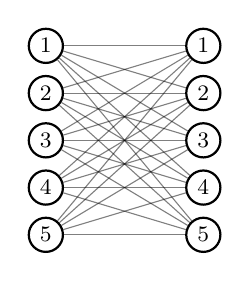
\begin{tikzpicture}
      \tikzstyle{every node} = [draw, circle, thick, inner sep = 2pt]
      \foreach \y in {0,...,4}{
        \pgfmathtruncatemacro{\yplusone}{5 - \y}
        \node(a\y) at (0,.6*\y) {\footnotesize\yplusone};
      }
      \foreach \y in {0,...,4}{
        \pgfmathtruncatemacro{\yplusone}{5 - \y}
        \node(\y) at (2,.6*\y) {\footnotesize\yplusone};
      }

      \foreach \x in {0,...,4}{
        \foreach \y in {0,...,4}{
          \path[opacity=0.5] (a\x) edge (\y);
        }
      }
    \end{tikzpicture}
  \end{center}
  \caption{Examples}
  \label{con_ex}
\end{figure}

\todo{Figure~\ref{con_ex}. It's just a placeholder right now}


Connectivity graphs also allow to graphically modelize how weights are tied in a neural layer. Let's suppose the $\Theta_ij$ are taking their values only into the finite set $K = \{w_1, w_2, \ldots, w_\kappa\}$ of size $\kappa$, which we will refer to as the \emph{kernel} of \emph{weights}. Then we can define a labelling of the edges $s: E \rightarrow K$. $s$ is called the \emph{weight sharing scheme} of the layer. This layer can then be formulated as $\displaystyle \forall v \in M, y_v = \sum_{u \in N, (u,v) \in E} w_{s(u,v)} x_u$. Figure~\ref{cnn} depicts the connectivity graph of a 1-d convolution layer and its weight sharing scheme.

\begin{figure}[h]
  \begin{center}
    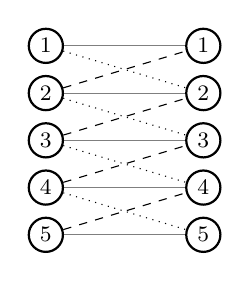
\begin{tikzpicture}
      \tikzstyle{every node} = [draw, circle, thick, inner sep = 2pt]
      \foreach \y in {0,...,4}{
        \pgfmathtruncatemacro{\yplusone}{5 - \y}
        \node(a\y) at (0,.6*\y) {\footnotesize\yplusone};
      }
      \foreach \y in {0,...,4}{
        \pgfmathtruncatemacro{\yplusone}{5 - \y}
        \node(\y) at (2,.6*\y) {\footnotesize\yplusone};
      }
      \path[opacity=0.5]
      (a0) edge (0);
      \path[dashed]
      (a0) edge (1);
      \path[dotted]
      (a1) edge (0);
      \path[opacity=0.5]
      (a1) edge (1);
      \path[dashed]
      (a1) edge (2);
      \path[dotted]
      (a2) edge (1);
      \path[opacity=0.5]
      (a2) edge (2);
      \path[dashed]
      (a2) edge (3);
      \path[dotted]
      (a3) edge (2);
      \path[opacity=0.5]
      (a3) edge (3);
      \path[dashed]
      (a3) edge (4);
      \path[dotted]
      (a4) edge (3);
      \path[opacity=0.5]
      (a4) edge (4);
    \end{tikzpicture}
  \end{center}
  \caption{Depiction of a 1D-convolutional layer and its weight sharing scheme.}
  \label{cnn}
\end{figure}


\todo{Add weight sharing scheme in Figure~\ref{cnn}}

\subsubsection{Computation graph}
\label{comp_graph}

\subsubsection{Underlying graph structure}
\label{inductive_graph}

\subsubsection{Graph-structured dataset}
\label{transductive_graph}

transductive vs inductive

\subsection{Geometric grids}

\subsection{Grid graphs}

\subsection{Spatial graphs}

\subsection{Projections of spatial graphs}

\end{document}